\section{Results and Discussion}
\label{sec:results}

\subsection{Compression Rate 64} \label{sec:compRate64}
To evaluate the results of the project in detail, we will consider the compression rate 64, as this is the highest compression rate with reasonable results.
In \Cref{fig:OriginalEncodedDecoded}, we can see $3$ example segments of the signal.
In \Cref{fig:OriginalEncodedDecoded1}, we can observe that a spike is preserved and that the noise in the signal is visibly reduced.
This implies that the autoencoder has the ability to correctly recognise a spike in the original data.
In \Cref{fig:OriginalEncodedDecoded2}, we see a segment of original data with no spikes and only noise. 
We can observe that output of the Decoder shows a significant smoothing of the signal.
Therefore, we can postulate that the autoencoder can remove noise.
Lastly, looking at \Cref{fig:OriginalEncodedDecoded3}, we can see how the autoencoder behaves, when the signal shows spikes of significant signal strength.
While the noise is still vastly removed, we can also observe that the spike becomes smaller regarding the signal strength. 
It should also be noted that the output of the Encoder does not necessarily have to be in the range $[0,1]$.
We also observe that the output of the Encoder does not fully reflect the shapes that can be found in both the input of the Encoder and the output of the Decoder.
\begin{figure}[h]
	\centering
	\begin{subfigure}[b]{\textwidth} 
		\centering
		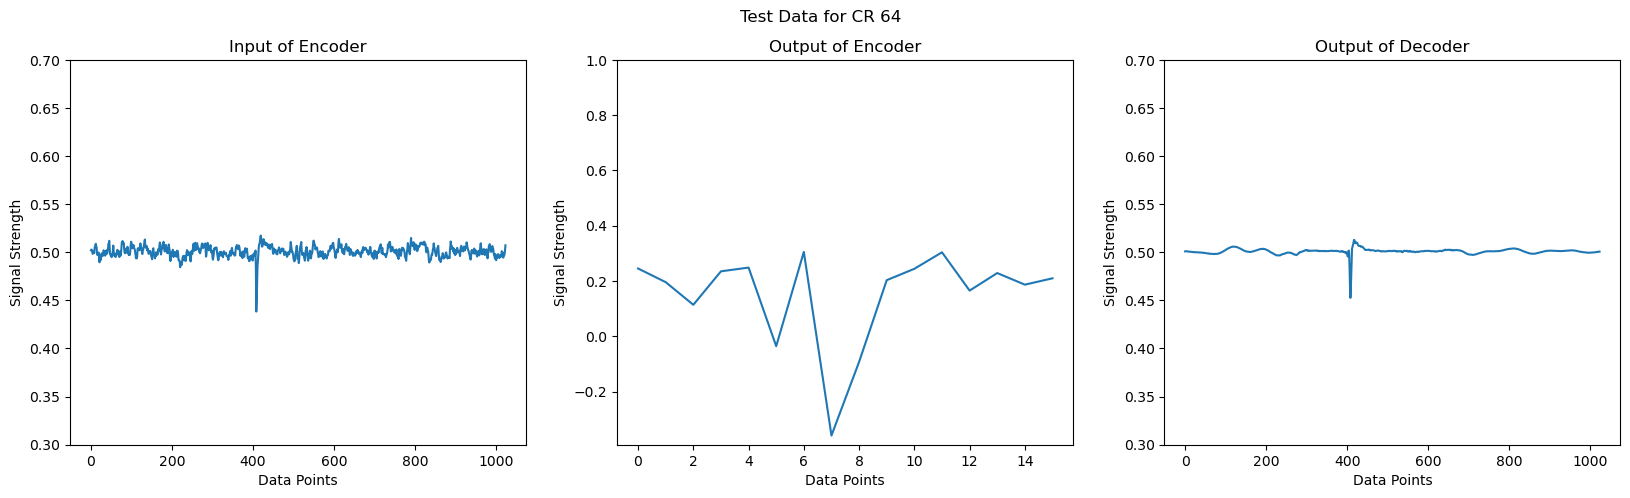
\includegraphics[width=\textwidth]{../../Images/EncodedDecodedCR64_1.png}
		\caption{Example 1}
		\label{fig:OriginalEncodedDecoded1}
	\end{subfigure}
	\begin{subfigure}[b]{\textwidth} 
	\centering
	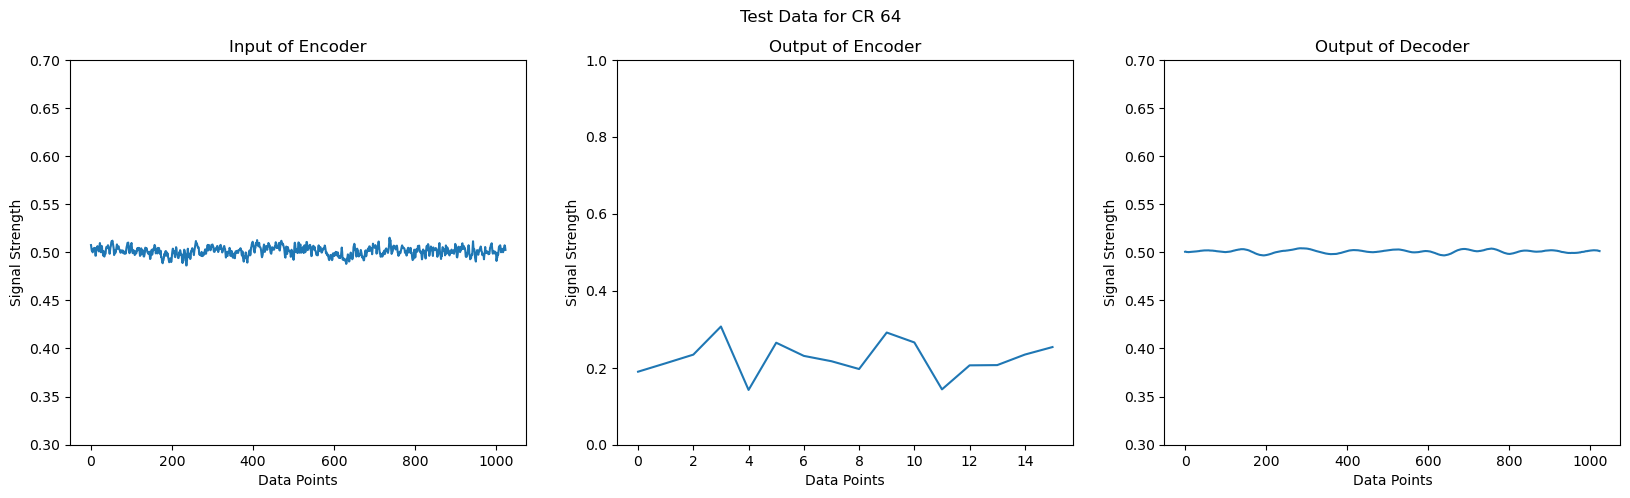
\includegraphics[width=\textwidth]{../../Images/EncodedDecodedCR64_2.png}
	\caption{Example 2}
	\label{fig:OriginalEncodedDecoded2}
	\end{subfigure}
	\begin{subfigure}[b]{\textwidth} 
	\centering
	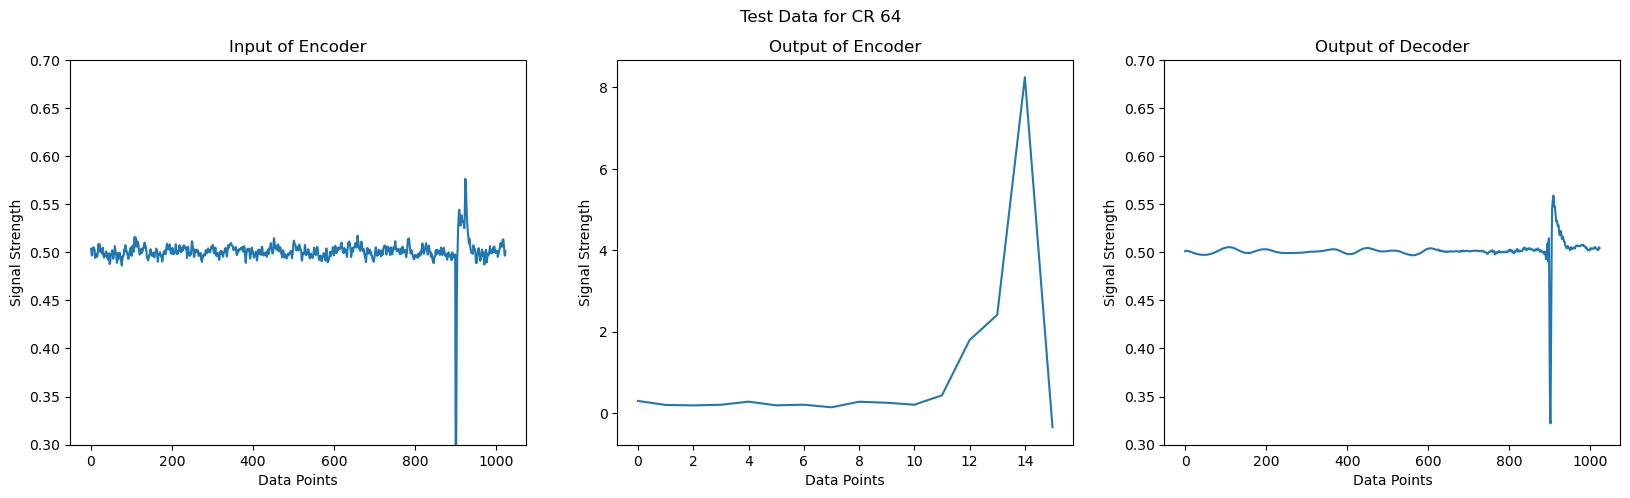
\includegraphics[width=\textwidth]{../../Images/EncodedDecodedCR64_3.png}
	\caption{Example 3}
	\label{fig:OriginalEncodedDecoded3}
	\end{subfigure}
	\caption{
		Every row of images shows how the autoencoder processes a given segment of the normalized raw signal (for a specific time section).
		For a compression rate 64, the amount of input and output data points is equal, as described in \Cref{sec:background}. Thus the output of the Encoder consists of $\frac{1024}{64} = 16$ data points. 		
	}
	\label{fig:OriginalEncodedDecoded}
\end{figure}
\FloatBarrier

In \Cref{fig:CrossingExample}, a section of the original signal and the decoded signal can be observed.
\Cref{fig:CrossingExample1} shows a few possible thresholds to evaluate the crossing point analysis, as described in \Cref{sec:thresholdAnalysis}.
In \Cref{fig:CrossingExample2}, we can see an example for detection of crossings for $2$ specific thresholds $0.45$ and $0.55$. 
The vertical lines indicate a crossing with the $2$ chosen thresholds.
On the basis of this information, we can infer the spike position in the original and decoded dataset.
For this specific compression rate and example, you can see that the crossings happen in the same place, and thus we have preserved crossings.
\begin{figure}[h]
	\centering
	\begin{subfigure}[t]{.49\textwidth} 
		\centering
		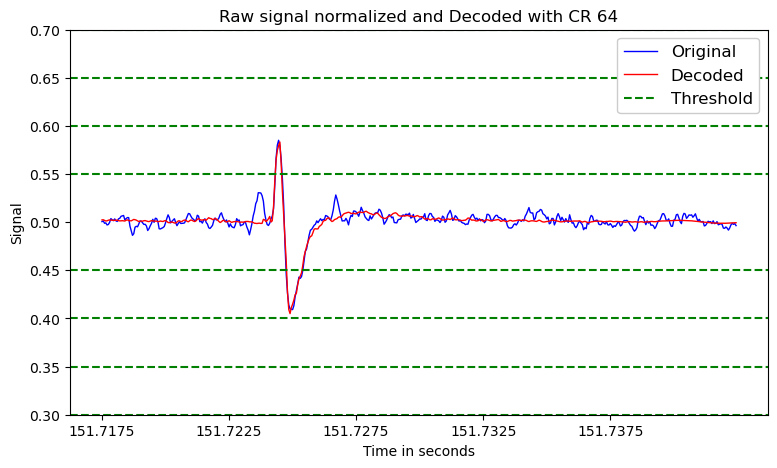
\includegraphics[width=\linewidth]{../../Images/Presentation_Segment_CR64_all_thresholds.png}
		\caption{Overview of a few possible thresholds. We choose increments of $0.05$ between the thresholds. The threshold $0.5$ is omitted, as it is too close to the mean of the signal and thus does not reflect any meaningful information.}
		\label{fig:CrossingExample1}
	\end{subfigure}
\hfill
	\begin{subfigure}[t]{.49\textwidth} 
		\centering
		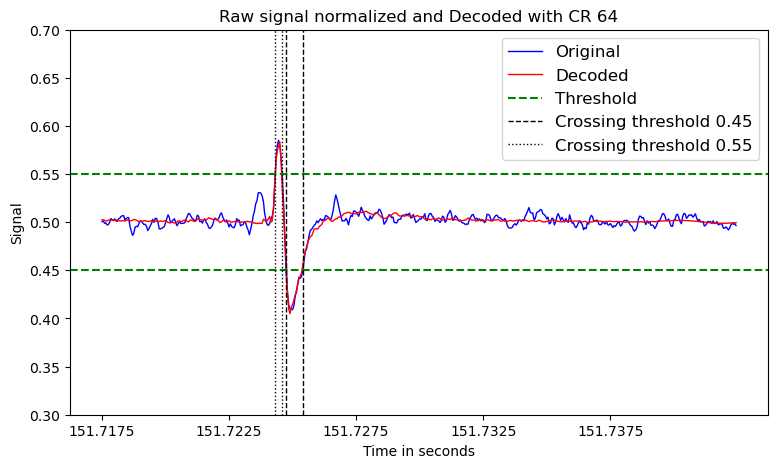
\includegraphics[width=\linewidth]{../../Images/Presentation_Segment_CR64_thresholds_drawn.png}
		\caption{Example for the crossing points analysis with the thresholds $0.45$ and $0.55$.}
		\label{fig:CrossingExample2}
	\end{subfigure}%
	\caption{Section of the raw normalized signal overlaid with the output of the autoencoder with CR 64 for the same segment of signal.}
	\label{fig:CrossingExample}
\end{figure}
\FloatBarrier

\subsection{Comparison of Compression Rates}
In the following we evaluate the influence of compression rates on the results, as described in \Cref{fig:CrTable}.
In \Cref{fig:CR2AndCR64}, we can see the differences in the decoded signal between compression rate $2$ and compression rate $64$ for the same section of input data.
We can observe that, for compression rate $2$ the shape of the original data is very well preserved (see \Cref{fig:CR2AndCR641}). This includes both the spike and the noise in the signal.
For compression rate $64$ (see \Cref{fig:CR2AndCR642}), we can see that the preservation is visibly worse, while the spike shape is being maintained, the structures that form the noise get simplified and smoothened.
This is in line with our expectations regarding different compression rates for the used autoencoders.

\begin{figure}[h]
	\centering
	\begin{subfigure}[b]{.49\textwidth}
		\centering
		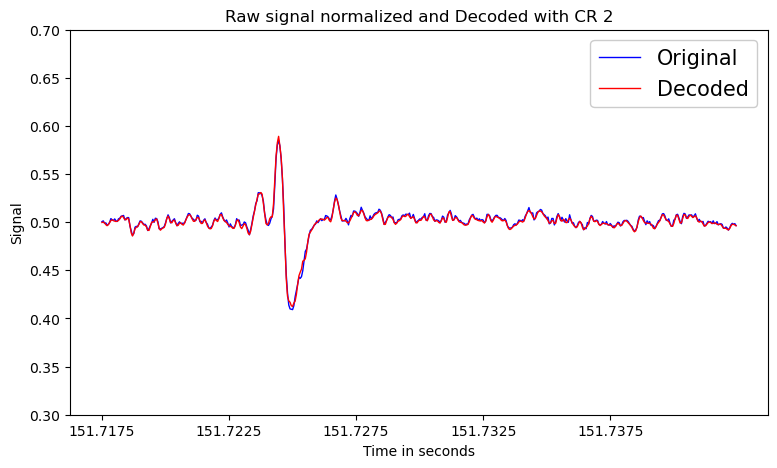
\includegraphics[width=\textwidth]{../../Images/Presentation_Segment_CR2.png}
		\caption{Example with compression rate $2$}
		\label{fig:CR2AndCR641}
	\end{subfigure}
\hfill
	\begin{subfigure}[b]{.49\textwidth}
		\centering
		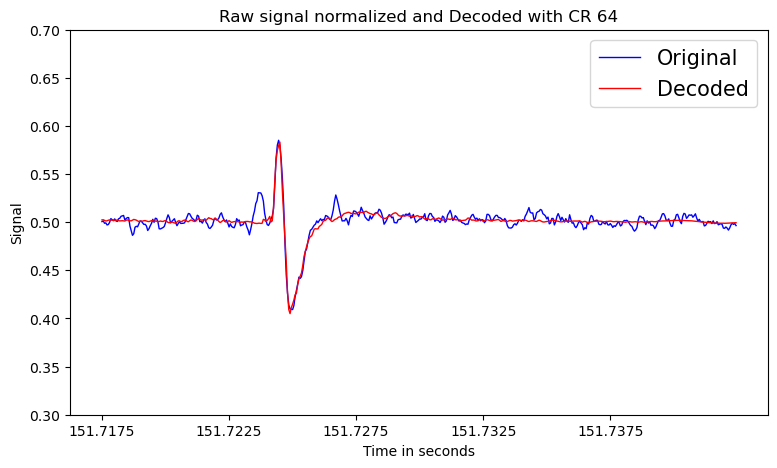
\includegraphics[width=\textwidth]{../../Images/Presentation_Segment_CR64.png}
		\caption{Example with compression rate $64$}
		\label{fig:CR2AndCR642}
	\end{subfigure}
	\caption{A section of the raw normalized signal overlaid with the output of autoencoder with different compression rates}
	\label{fig:CR2AndCR64}
\end{figure}
\FloatBarrier

The observation that higher compression rates preserve the structures in the original signal worse is also supported by \Cref{fig:mse} and \Cref{fig:snr}.
Here, we can see that the MSE grows approximately logarithmically with increasing compression rate.
We can also see that the SNR decreases with an increase in compression rate.
This is also in line with our expectations, as a higher compression rate results in less information being able to pass through the bottleneck layer.

\begin{figure}[h]
	\begin{subfigure}{.48\textwidth}
		\centering
		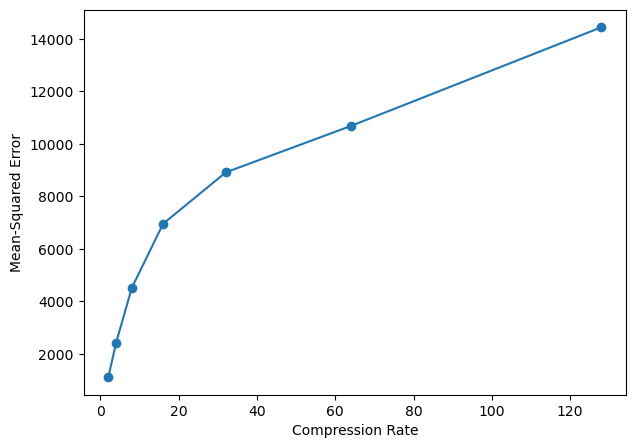
\includegraphics[width=1\linewidth]{../../Images/mse.png}
		\caption{MSE, as defined in \Cref{eq:mse}, for the different used compression rates.}
		\label{fig:mse}
	\end{subfigure} \hfill
	\begin{subfigure}{.48\textwidth}
		\centering
		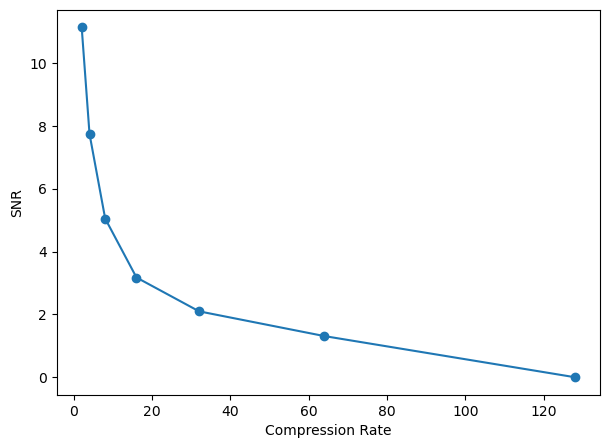
\includegraphics[width=1\linewidth]{../../Images/snr.png}
		\caption{SNR, as defined in \Cref{eq:snr}, for the different used compression rates.}
		\label{fig:snr}
	\end{subfigure}
\caption{The MSE and the SNR is calculated between the raw input and the output signal of the respective autoencoders implementing the shown compression rates for the whole test subset}
\label{fig:msesnr}
\end{figure}
\FloatBarrier

In \Cref{fig:DecodedBarChar}, we can observe the calculated number of crossings for two different exemplary thresholds for the whole test subset.
The number of preserved crossings can help us understand the quality of spike preservation and thus spike detection of the respective autoencoder.
Note that the crossings detected in the decoded data are not always the same as the ones in the original data. 
This is reflected in the difference between the number of decoded data crossings and preserved crossings.
Firstly, we observe that the original data always has a higher number of crossings than any decoded data. 
This suggests that the use of autoencoders in our case leads to a loss of information about the signal.
In \Cref{fig:DecodedBarChar1}, we can see that for threshold $0.45$ compression rate $4$ yields worse results than the next higher evaluated compression rate of $8$.
This is a surprising observation.
However, it can be generally said that with an increase in compression rate, we achieve worse results regarding the number of decoded crossings, as well as preserved crossings.
For threshold $0.55$ (see \Cref{fig:DecodedBarChar2}), the decreasing number of crossings for increasing compression rates is maintained.
This is also consistent with other thresholds, as can be seen in \Cref{appendix:ThresholdAnalysis}.
Also note that compression rate $64$ is the highest compression rate which yields sensible results.
Compression rate $128$ does not include any crossings and thus does not preserve any information from the original dataset.

\begin{figure}[h]
	\centering
	\begin{subfigure}{.5\textwidth}
		\centering
		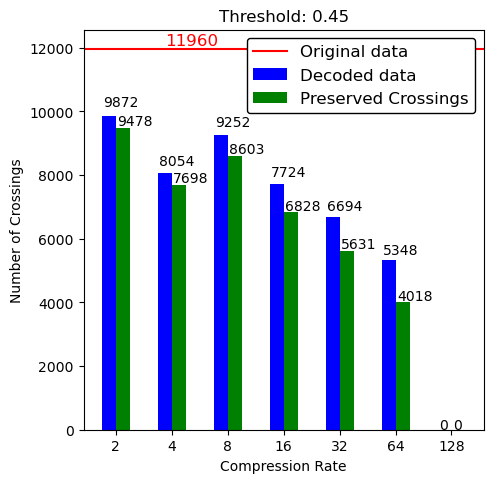
\includegraphics[width=\linewidth]{../../Images/spikes_threshold_045.png}
		\caption{Example for the threshold $0.45$}
		\label{fig:DecodedBarChar1}
	\end{subfigure}\hfill 
	\begin{subfigure}{.5\textwidth}
		\centering
		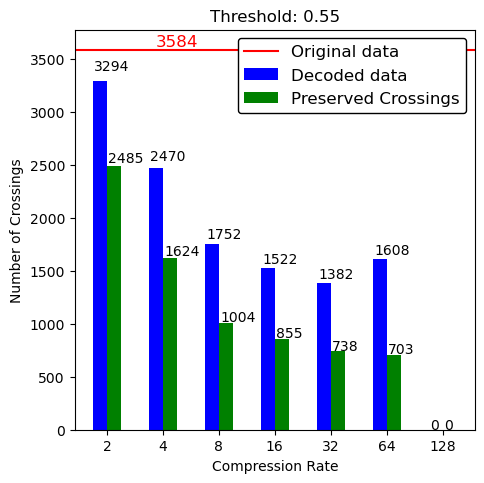
\includegraphics[width=\linewidth]{../../Images/spikes_threshold_055.png}
		\caption{Example for the threshold $0.55$}
		\label{fig:DecodedBarChar2}
	\end{subfigure}
	\caption{Bar charts for different compression rates illustrating the number of crossings in the original data, the decoded data and the number of preserved crossings, as described in \Cref{sec:thresholdAnalysis}}.
	\label{fig:DecodedBarChar}
\end{figure}
\FloatBarrier

Lastly, we analyze the percentage of correctly preserved crossings for different thresholds and compression rates, as seen in \Cref{fig:percentageDecodedLineChart}.
Generally, it can be observed that a higher compression rate yields a lower percentage of correctly preserved crossings, with the autoencoder implementing compression rate $128$ maintaining $0$ correctly preserved crossings for every threshold.
It is important to notice that the behavior of the autoencoder implementing compression rate $4$ shows surprising character.
Specifically, for thresholds less than $0.5$, it yields worse results than expected.
The percentages of preserved crossings are lower than the ones for compression rate $8$ for thresholds less than $0.5$.
On the other hand, the autoencoder for compression rate $4$ outperforms the one for compression rate $8$ for thresholds bigger than $0.5$.
Generally, it can again be said, that with an increase in compression rate, the autoencoder performs worse.
A further observation is that for thresholds close to the edges of the interval $[0,1]$ our respectively used autoencoders yield worse results.
This is expected, as we have fewer crossings in total with such extreme values.
Further, this supports our earlier observation in \Cref{sec:compRate64} that spikes become smaller regarding the signal strength when processed with the used autoencoders.
This claim is also supported by the threshold analysis images provided in \Cref{appendix:ThresholdAnalysis}.

\begin{figure}[h]
	\centering
	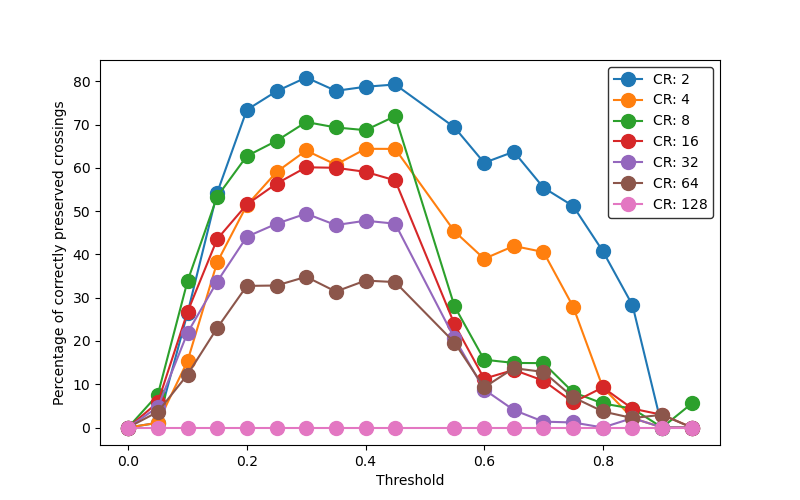
\includegraphics[width=\linewidth]{../../Images/percentage_decoded.png}
	\caption{Line graph showing the percentage of correctly preserved crossings, as defined in \Cref{eq:percCorrectlyPreservedCrossings}. 
	Compression rate values are represented by different colors}.
	\label{fig:percentageDecodedLineChart}
\end{figure}
\FloatBarrier